\documentclass[aspectratio=169,11pt]{beamer}
\usepackage[utf8]{inputenc}
\usepackage[T1]{fontenc}
\usepackage{mathptmx}
\usepackage{graphicx}
\usepackage{booktabs}
\usepackage{amsmath}
\usepackage{url}
\usepackage[export]{adjustbox}

\usetheme{Madrid}
\definecolor{navy}{RGB}{23,50,95}
\definecolor{teal}{RGB}{0,128,128}
\definecolor{risk}{RGB}{200,60,50}
\setbeamercolor{palette primary}{bg=navy,fg=white}
\setbeamercolor{palette secondary}{bg=navy!85,fg=white}
\setbeamercolor{palette tertiary}{bg=navy!70,fg=white}
\setbeamercolor{structure}{fg=navy}
\setbeamercolor{block title}{bg=navy,fg=white}
\setbeamercolor{block body}{bg=navy!6}
\setbeamertemplate{navigation symbols}{}
\setbeamertemplate{footline}[frame number]
\newcommand{\code}[1]{\texttt{\small #1}}

\title[Predicting Loan Default]{Predicting Loan Default on Lending Club Data}
\subtitle{Application-time scoring with out-of-time validation}
\author[Group]{\textbf{[Student 1]}, \textbf{[Student 2]}}
\institute[NEU]{School of Technology, National Economics University\\ Statistical Learning (DS66A / DS66B) \quad|\quad Supervisor: [Name]}
\date{\today}
\titlegraphic{
\includegraphics[height=1.4cm]{Images/Logo-NEU.png}}

\begin{document}

\begin{frame}[plain]
\titlepage
\end{frame}

\begin{frame}{Outline}
\begin{columns}[T]
\column{0.5\textwidth}
\begin{enumerate}
\item Problem statement
\item Objectives and contributions
\item Data and target definition
\item Out-of-time split
\item Leakage control and cleaning
\item Feature selection and engineering
\end{enumerate}
\column{0.5\textwidth}
\begin{enumerate}
\setcounter{enumi}{6}
\item Models, tuning and metrics
\item Validation and test results
\item Experiment 1: without \code{sub\_grade}
\item Experiment 2: compact scorecard
\item Conclusion, limitations, future work
\end{enumerate}
\end{columns}
\end{frame}

\section{Problem}
\begin{frame}{Problem statement}
\begin{columns}[T]
\column{0.58\textwidth}
\textbf{Lending Club} (US peer-to-peer lending) published its loan records. Each loan ends as \alert{Charged Off} (default, label 1) or \alert{Fully Paid} (label 0).

\medskip
\textbf{Question.} Using only information known at application time, how well can we \emph{rank} applicants by default risk, and does a model beat the platform's own \code{sub\_grade} (A1 to G5)?

\medskip
\textbf{Why it is hard}
\begin{itemize}
\item \textbf{Leakage}: many of the 151 columns are created after the loan starts
\item \textbf{Time}: default rate drifts (13.7\% $\rightarrow$ 14.8\%)
\item \textbf{Censoring}: recent loans have no final outcome yet
\item \textbf{Incumbent}: \code{sub\_grade} is already a risk model
\end{itemize}
\column{0.4\textwidth}
\begin{block}{Task}
\textbf{Input}: borrower and credit-bureau data at application\\
\textbf{Output}: score $p\in[0,1]$, the estimated probability of default, used to rank loans\\
\textbf{Label}: Charged Off $=1$, Fully Paid $=0$
\end{block}
\begin{alertblock}{Key rule}
No data created after approval.
\end{alertblock}
\end{columns}
\end{frame}

\begin{frame}{Objectives and contributions}
\textbf{Objective:} estimate honestly how much application-time information adds to \code{sub\_grade} for ranking default risk.

\medskip
\begin{block}{Contributions}
\begin{itemize}
\item Leakage-controlled protocol: application-time whitelist, evidence from single-column AUC
\item Out-of-time 70/15/15 split on matured 36-month loans, with a fixed split manifest
\item Pipeline fitted on train only (median impute, scaling, one-hot)
\item Comparison of baseline, Logistic L2, Decision Tree, Random Forest, HistGB with ROC-AUC, Gini, KS and paired bootstrap
\item Two follow-ups: removing \code{sub\_grade}, and a compact 12-field scorecard
\item Negative results reported as they are
\end{itemize}
\end{block}
\end{frame}

\section{Data}
\begin{frame}{Data dictionary: which columns are known at application?}
\begin{columns}[T]
\column{0.5\textwidth}
Kaggle file: \textbf{2,260,701} loans, \textbf{151} columns (2007--2018). Every column is tagged with a hypothesis.

\medskip
\adjustbox{max width=\linewidth}{\begin{tabular}{lr}
\toprule
Group & Columns\\
\midrule
Credit history (1) & 38\\
Credit history (2) & 31\\
Loan information & 21\\
Joint application & 16\\
Post-loan payments & 15\\
Hardship plan & 15\\
Borrower information & 8\\
Debt settlement & 7\\
\bottomrule
\end{tabular}}
\column{0.46\textwidth}
\begin{block}{Timing tags}
\textbf{Yes}: 103 known at application\\
\textbf{No}: 41 after the loan, or identifiers\\
\textbf{Uncertain}: 7 timing unclear
\end{block}
\begin{itemize}
\item Dictionary matches the raw header: 151 / 151, none missing, extra or duplicated
\item The tags are \alert{hypotheses}; they are tested with data later (single-column AUC)
\end{itemize}
\end{columns}
\end{frame}

\begin{frame}{Target and population}
\begin{columns}[T]
\column{0.5\textwidth}
\textbf{Label} from \code{loan\_status}: Fully Paid $\to 0$, Charged Off $\to 1$. A loan is final only if no principal is outstanding (checked with \code{out\_prncp}).

\medskip
\textbf{Filters (each verified by code)}
\begin{itemize}
\item labelled
\item issued from 2012 (pre-2012 is 2.96\% of labelled loans; 44 numeric columns start in 2012)
\item \alert{matured}: issue month + term $\le$ 2018-12 (99.6\% of matured loans are labelled vs 42.4\%)
\item 36-month term (all three sets share one term)
\end{itemize}
\column{0.48\textwidth}
\adjustbox{max width=\linewidth}{\begin{tabular}{lrr}
\toprule
Step & Rows & Kept\\
\midrule
Raw data & 2,260,701 & 100\%\\
Labelled & 1,345,310 & 59.5\%\\
From 2012 & 1,305,524 & 57.7\%\\
Matured & 633,767 & 28.0\%\\
\textbf{36-month} & \textbf{589,488} & \textbf{26.1\%}\\
\bottomrule
\end{tabular}}

\medskip
Among labelled loans: 80.0\% Fully Paid, 20.0\% Charged Off (14.0\% after filtering).
\end{columns}
\end{frame}

\begin{frame}{Out-of-time split: train on the past, test on the future}
\begin{columns}[T]
\column{0.42\textwidth}
\adjustbox{max width=\linewidth}{\begin{tabular}{lrcc}
\toprule
Set & Rows & Period & Default\\
\midrule
Train & 408,188 & 2012-01 to 2015-05 & 13.7\%\\
Val & 92,631 & 2015-06 to 09 & 14.7\%\\
Test & 88,669 & 2015-10 to 12 & 14.8\%\\
\bottomrule
\end{tabular}}

\medskip
\begin{itemize}
\item Sort by issue date; cut at the dates found at 70\% and 85\% of rows
\item Whole months stay in one set; assertions check train $<$ val $<$ test
\item Default rate drifts up $+1.1$ points
\item Manifest stores an MD5 of train ids
\end{itemize}
\column{0.56\textwidth}
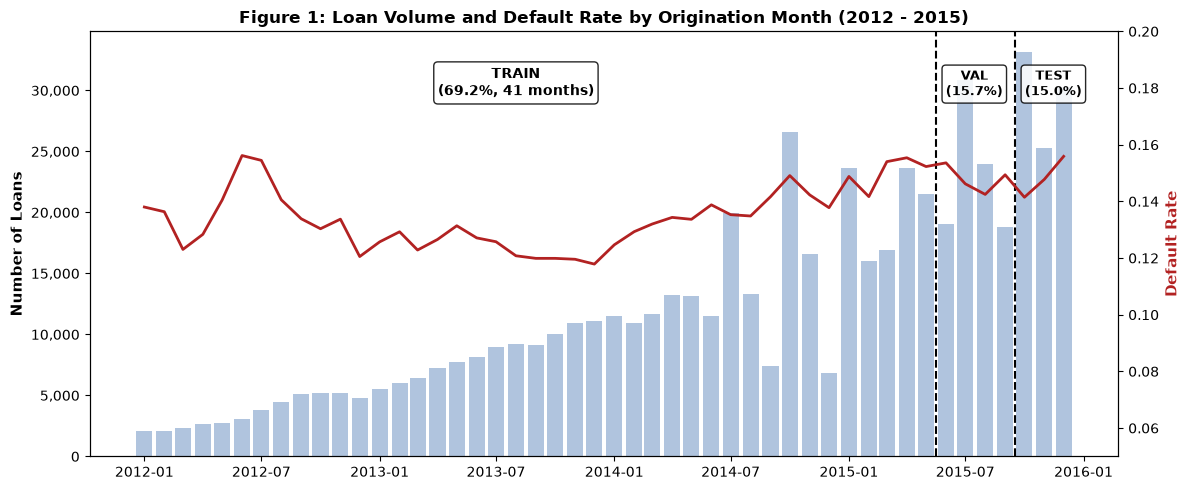
\includegraphics[width=\linewidth]{Images/time_split.png}
\end{columns}
\end{frame}

\section{Preparation}
\begin{frame}{Leakage control and cleaning}
\begin{columns}[T]
\column{0.5\textwidth}
\begin{block}{Six cleaning rules (row by row)}
\begin{itemize}
\item \code{annual\_inc} $\le0$, \code{loan\_amnt} $\le0$ $\to$ missing
\item \code{dti} outside 0--100 $\to$ missing
\item \code{revol\_util} capped at 102.4 (train 99.9th pct)
\item FICO low $>$ high $\to$ both missing
\item first credit line after issue date $\to$ missing
\end{itemize}
\end{block}
\column{0.48\textwidth}
\begin{alertblock}{Anti-leakage rules}
\begin{enumerate}
\item Split first, transform later
\item Median, mean, std, caps, categories: \textbf{train only}
\item Pipeline \code{fit} on train; val and test only \code{transform}
\item Same cleaning function on all three sets
\end{enumerate}
\end{alertblock}
Evidence: after scaling, train means are $\approx 0$ but validation means reach 0.162, because validation uses train statistics.
\end{columns}
\end{frame}

\begin{frame}{Feature selection: 151 $\rightarrow$ 57 columns}
\begin{columns}[T]
\column{0.4\textwidth}
\adjustbox{max width=\linewidth}{\begin{tabular}{lr}
\toprule
Rule (in order) & Columns\\
\midrule
Raw columns & 151\\
Label and helper & $-2$\\
Identifier & $-2$\\
Empty in train & $-32$\\
After loan / unclear & $-42$\\
Text $>100$ values & $-4$\\
Near constant & $-7$\\
Missing $>30\%$ & $-5$\\
\textbf{Candidates} & \textbf{57}\\
\bottomrule
\end{tabular}}
\column{0.58\textwidth}
\textbf{Leakage check: single-column ROC-AUC on train}

Best application-time column: \code{sub\_grade}, \textbf{0.6565}.

\adjustbox{max width=\linewidth}{\begin{tabular}{lr}
\toprule
Suspect column & AUC\\
\midrule
\code{last\_fico\_range\_low} & 0.9074\\
\code{recoveries} & 0.9054\\
\code{collection\_recovery\_fee} & 0.8677\\
\code{total\_rec\_prncp} & 0.8280\\
\code{total\_pymnt} & 0.7554\\
\bottomrule
\end{tabular}}

10 of the 42 suspect columns beat the best legitimate column: the whitelist is justified.
\end{columns}
\end{frame}

\begin{frame}{Feature engineering and pipeline: 57 $\rightarrow$ 153 columns}
\begin{columns}[T]
\column{0.5\textwidth}
\textbf{New features:} \code{fico\_avg}, \code{loan\_to\_income} (cap 0.5), \code{log\_annual\_inc}, \code{log\_revol\_bal}, \code{emp\_length\_years} (and \code{credit\_history\_years}, later dropped for $r=0.92$).

\medskip
\textbf{Dropped:} replaced columns, \code{grade} and \code{int\_rate} (duplicate \code{sub\_grade}), and 5 columns with $|r|\ge0.90$.

\medskip
\textbf{Result:} 45 numeric + 5 categorical $=$ 50 inputs $\rightarrow$ \textbf{153} columns after one-hot (108 dummies: \code{addr\_state} 50, \code{sub\_grade} 35, \code{purpose} 14, \code{home\_ownership} 6, \code{verification} 3).
\column{0.48\textwidth}
\begin{block}{Why median and scaling?}
\begin{itemize}
\item 28 of 31 columns with missing values are right-skewed; mean is pulled up (e.g. \code{avg\_cur\_bal}: mean 12,503 vs median 6,228)
\item Scales differ by $>10^5$ (0.34 to 127,162), which matters for the L2 penalty
\end{itemize}
\end{block}
\code{Pipeline: clean $\to$ features $\to$ ColumnTransformer(median+StandardScaler | OneHot)}
\end{columns}
\end{frame}

\begin{frame}{Default rate by decile (train): signal and non-linearity}
\begin{columns}[T]
\column{0.64\textwidth}
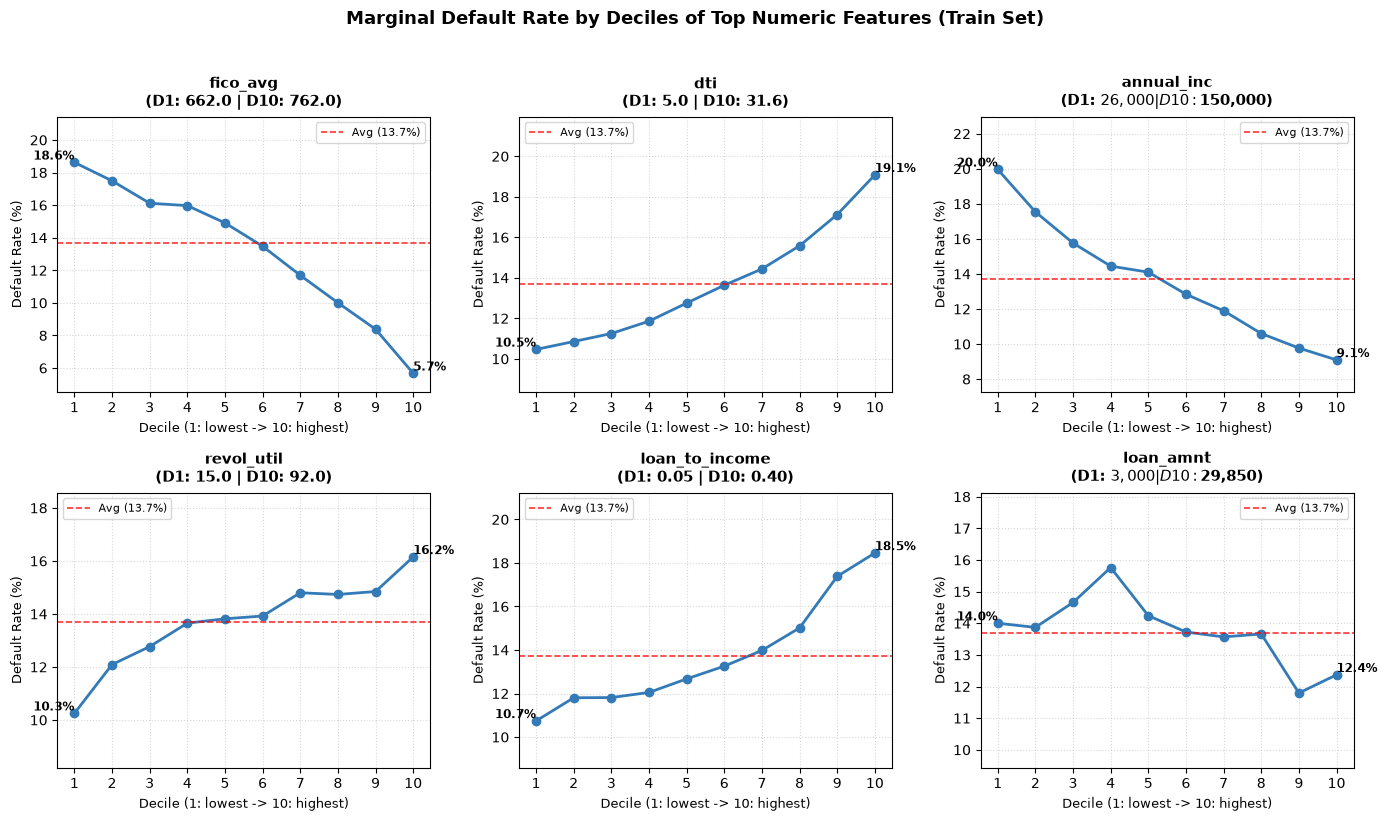
\includegraphics[width=\linewidth]{Images/decile.png}
\column{0.34\textwidth}
\begin{itemize}
\item FICO, income: risk falls steadily
\item DTI, utilisation, loan-to-income: risk rises
\item \code{loan\_amnt} is \alert{not monotone} (peak 15.7\%), which a linear term cannot capture
\item \code{sub\_grade}: default rate rises from 2.7\% (A1) to 36.4\% (G5)
\end{itemize}
\end{columns}
\end{frame}

\section{Models}
\begin{frame}{Models, tuning and metrics}
\begin{columns}[T]
\column{0.52\textwidth}
\textbf{Five models, 153 inputs} (baseline uses \code{sub\_grade} only). Tuned by \code{GridSearchCV} with \code{TimeSeriesSplit(3)} \alert{inside train}.

\medskip
\small
\adjustbox{max width=\linewidth}{\begin{tabular}{lll}
\toprule
Model & Selected & CV AUC\\
\midrule
Logistic L2 & $C=1$ & 0.6855\\
Decision Tree & depth 7 & 0.6355\\
Random Forest & 150 trees, depth 10 & 0.6741\\
HistGB & 150 iter, depth 10, lr 0.05 & 0.6852\\
\bottomrule
\end{tabular}}
\column{0.46\textwidth}
\begin{block}{Metrics (ranking, no threshold)}
\textbf{ROC-AUC}: chance a defaulter scores above a repaid loan\\
\textbf{Gini} $=2\,\mathrm{AUC}-1$\\
\textbf{KS} $=\max(\mathrm{TPR}-\mathrm{FPR})$
\end{block}
\begin{itemize}
\item Overfit check: AUC train $-$ AUC val
\item Paired bootstrap, $B=1{,}000$, 95\% CI of $\Delta$AUC
\item Test used once
\end{itemize}
\end{columns}
\end{frame}

\section{Results}
\begin{frame}{Validation results (92,631 loans)}
\begin{columns}[T]
\column{0.44\textwidth}
\small
\adjustbox{max width=\linewidth}{\begin{tabular}{lcccc}
\toprule
Model & AUC & Gap & Gini & KS\\
\midrule
Baseline & 0.6815 & $-0.025$ & 36.3\% & 27.0\%\\
Logistic & 0.7040 & $-0.017$ & 40.8\% & 29.9\%\\
Tree & 0.6536 & $+0.001$ & 30.7\% & 22.3\%\\
Random Forest & 0.6876 & $+0.018$ & 37.5\% & 27.2\%\\
HistGB & 0.7054 & $+0.004$ & 41.1\% & 30.0\%\\
\bottomrule
\end{tabular}}

\medskip
\textbf{Bootstrap $\Delta$AUC vs baseline}
\begin{itemize}
\item Logistic $+0.0225$ [+0.0196, +0.0253]
\item HistGB $+0.0238$ [+0.0206, +0.0270]
\item RF $+0.0061$ [+0.0024, +0.0102]
\item Tree $-0.0280$ [$-0.0329$, $-0.0233$]
\end{itemize}
\column{0.54\textwidth}
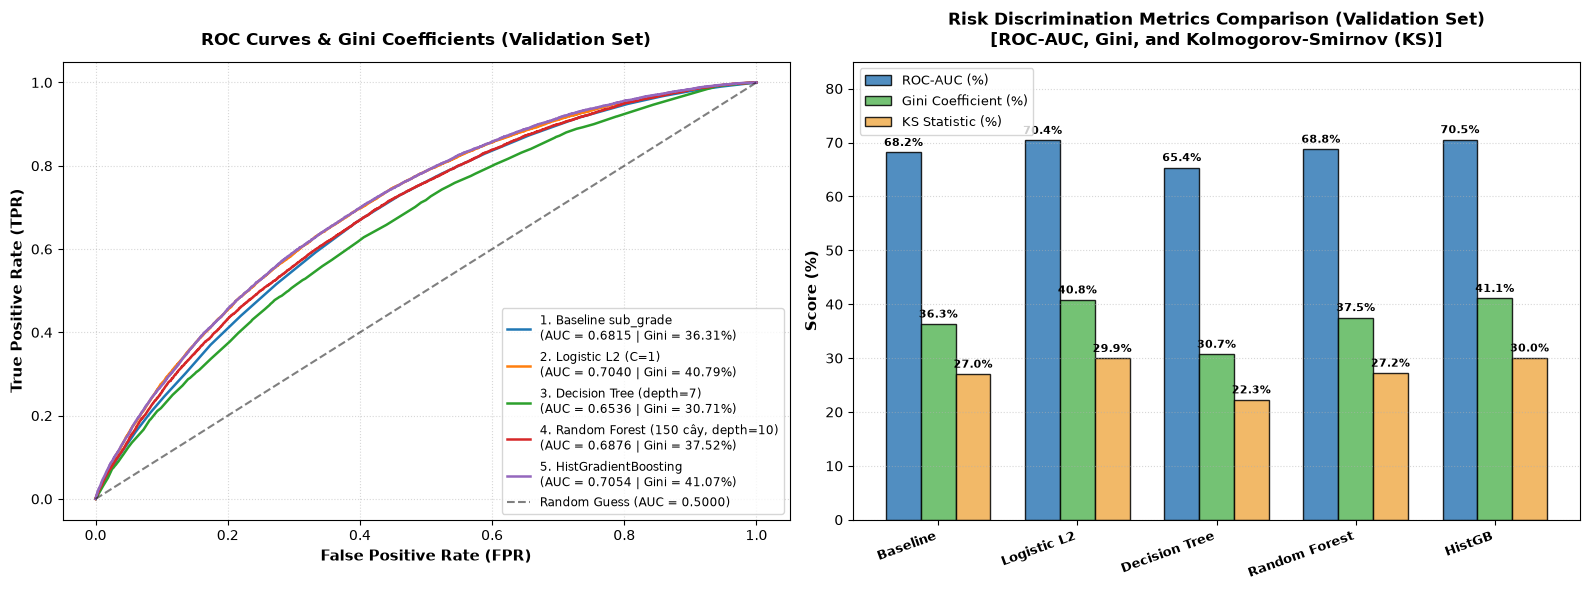
\includegraphics[width=\linewidth]{Images/model_comparison.png}
\end{columns}
\end{frame}

\begin{frame}{Out-of-time test and decision}
\begin{columns}[T]
\column{0.55\textwidth}
Test: 88,669 loans (2015-10 to 12), evaluated \alert{once}.

\medskip
\adjustbox{max width=\linewidth}{\begin{tabular}{lcccc}
\toprule
Model & AUC & Gini & KS & $\Delta$AUC\\
\midrule
Baseline \code{sub\_grade} & 0.6818 & 36.4\% & 26.5\% & ---\\
\textbf{Logistic L2} & \textbf{0.7039} & 40.8\% & 29.9\% & $+0.0221$\\
HistGB & 0.7055 & 41.1\% & 30.0\% & $+0.0237$\\
\bottomrule
\end{tabular}}

\medskip
HistGB $-$ Logistic on validation: 95\% CI [$-0.0002$, $+0.0031$] contains 0, so no real difference.
\column{0.42\textwidth}
\begin{block}{Decision: Logistic L2}
\begin{itemize}
\item beats baseline by $+0.022$ AUC
\item same level as HistGB
\item fast, no overfitting
\item each coefficient is explainable
\end{itemize}
\end{block}
Choosing Logistic is a modelling judgement, not a statistical result.
\end{columns}
\end{frame}

\begin{frame}{Experiment 1: remove \code{sub\_grade} (153 $\rightarrow$ 118 features)}
\begin{columns}[T]
\column{0.42\textwidth}
\small
\adjustbox{max width=\linewidth}{\begin{tabular}{lccc}
\toprule
Model & Val AUC & Test AUC & Test KS\\
\midrule
Baseline & 0.6815 & 0.6818 & 26.5\%\\
Logistic, with & 0.7040 & 0.7039 & 29.9\%\\
Logistic, without & 0.6890 & 0.6879 & 27.3\%\\
\bottomrule
\end{tabular}}

\medskip
\begin{itemize}
\item Without the grade, still above baseline: $+0.0075$ [+0.0033, +0.0117]
\item \code{sub\_grade} adds $+0.0150$ [+0.0133, +0.0167]
\item Coefficients grow when the grade is removed: \code{fico\_avg} $2.2\times$, \code{log\_annual\_inc} $2.6\times$, \code{revol\_util} $1.9\times$
\end{itemize}
\column{0.56\textwidth}
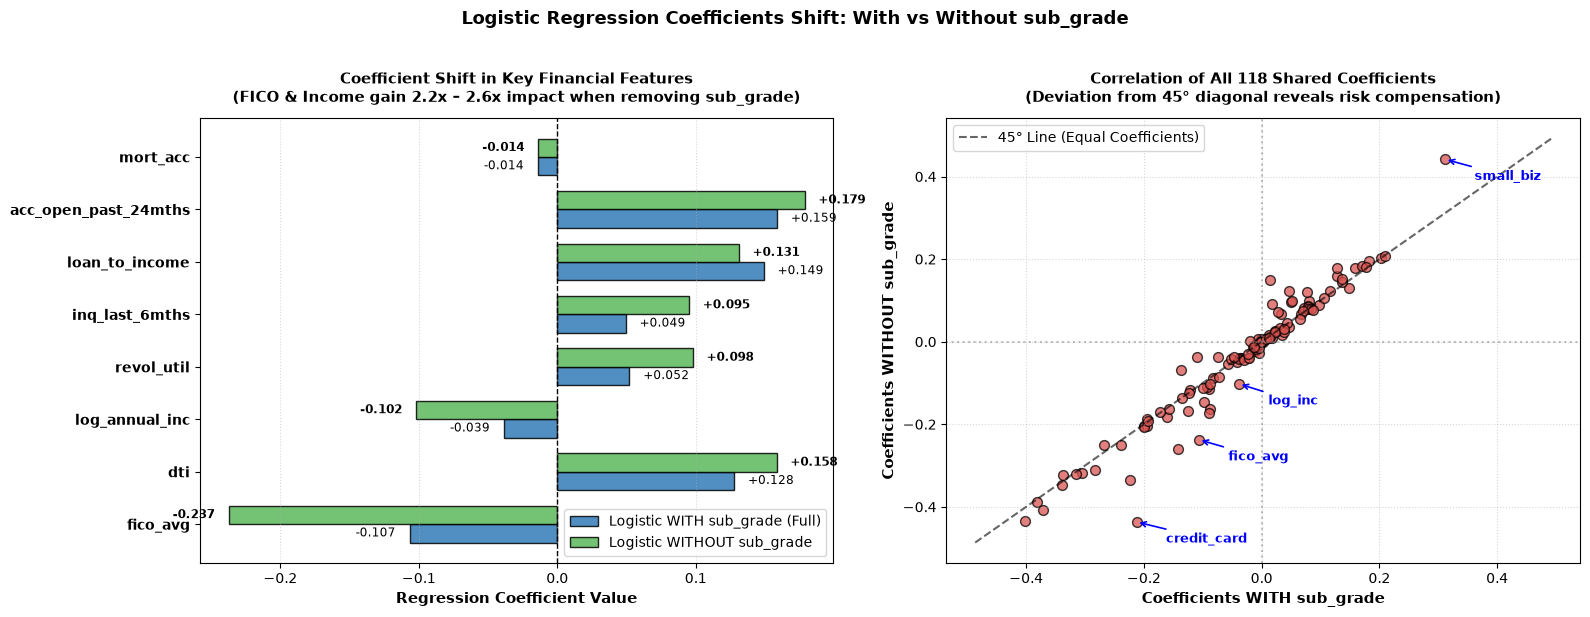
\includegraphics[width=\linewidth]{Images/coef_shift.png}

\footnotesize The grade absorbs signal from these variables (association, not causation).
\end{columns}
\end{frame}

\begin{frame}{Experiment 2: compact 12-field scorecard}
\begin{columns}[T]
\column{0.4\textwidth}
\small
\adjustbox{max width=\linewidth}{\begin{tabular}{lccc}
\toprule
Model & Cols & Test AUC & Gini\\
\midrule
Full Logistic & 153 & 0.7039 & 40.8\%\\
Compact & 30 & 0.6730 & 34.6\%\\
\bottomrule
\end{tabular}}

\medskip
Compact keeps 84.8\% of the full Gini with 80\% fewer columns but is \alert{below the baseline} (0.6818).

\medskip
\textbf{Score}: $\text{Offset}-\text{Factor}\cdot\ln(\text{odds})$, Factor $=\mathrm{PDO}/\ln2$; PDO 20, 600 points at odds 1/5 (conventions we chose).

\medskip
\adjustbox{max width=\linewidth}{\begin{tabular}{lcc}
\toprule
Band & Share & Default\\
\midrule
$<590$ & 11.4\% & 30.2\%\\
590--614 & 47.6\% & 17.3\%\\
615--639 & 33.5\% & 8.7\%\\
$\ge640$ & 7.5\% & 3.3\%\\
\bottomrule
\end{tabular}}
\column{0.58\textwidth}
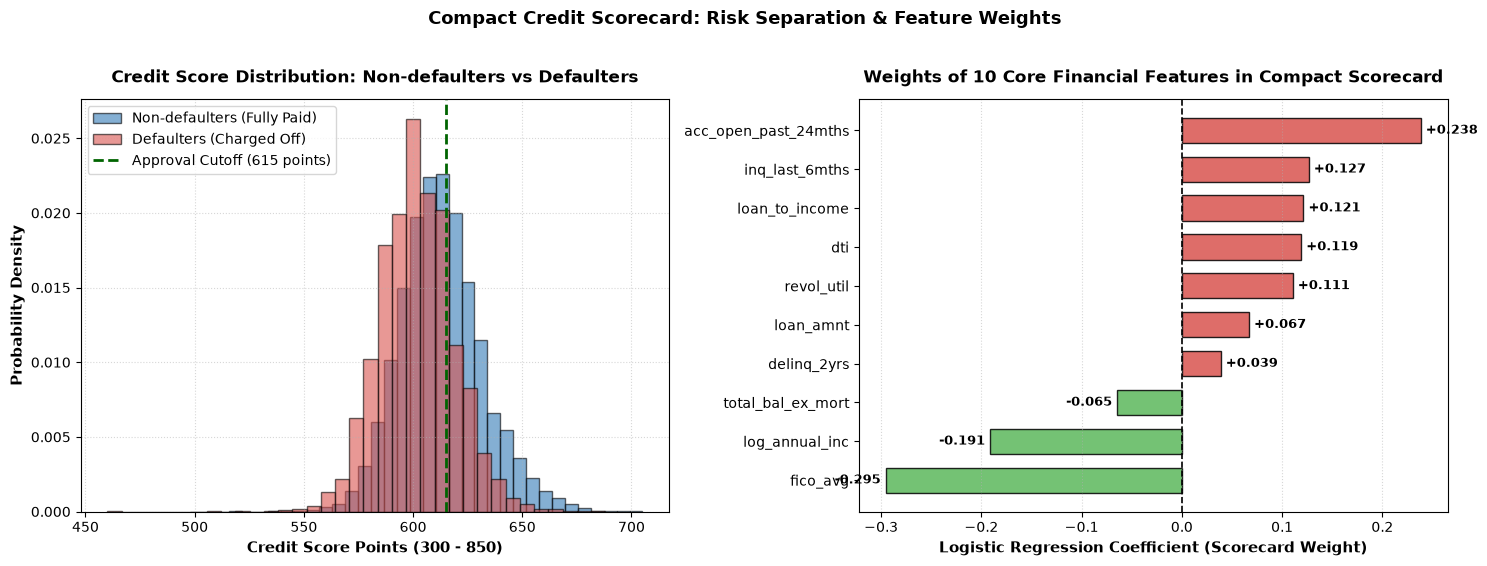
\includegraphics[width=\linewidth]{Images/scorecard.png}

\footnotesize Test set; cut-offs set on validation.
\end{columns}
\end{frame}

\section{Conclusion}
\begin{frame}{Conclusion}
\begin{enumerate}
\item \textbf{The incumbent is beaten, modestly.} Test AUC: baseline 0.6818, Logistic 0.7039, HistGB 0.7055; intervals on validation exclude zero.
\item \textbf{More complex is not clearly better.} HistGB and Logistic tie; the forest gains less; a depth-7 tree loses to the baseline.
\item \textbf{The grade absorbs signal.} Without \code{sub\_grade}: test AUC 0.6879 ($+0.0061$ over baseline); FICO and income coefficients about double.
\item \textbf{A compact scorecard is cheap but weaker}, yet separates risk bands from 30.2\% to 3.3\% observed default.
\item Every number is printed by code on real data, and disappointing results are reported as such.
\end{enumerate}
\end{frame}

\begin{frame}{Limitations and future work}
\begin{columns}[T]
\column{0.5\textwidth}
\begin{block}{Limitations}
\begin{itemize}
\item 36-month loans of 2012--2015; three-month test window
\item Random Forest and HistGB grids hit their edges
\item Bootstrap CI covers validation sampling only
\item Val AUC $>$ train AUC for the baseline and Logistic: observed, not explained
\item No calibration, thresholds or cost analysis
\item Scorecard constants (600, PDO 20) are conventions
\end{itemize}
\end{block}
\column{0.48\textwidth}
\begin{block}{Future work}
\begin{itemize}
\item Wider or randomised hyperparameter search
\item Rolling-origin evaluation and dataset-shift tests \cite{qian2021}
\item Missing-indicator treatment of \code{mths\_since\_...} columns
\item Calibration and cost-sensitive thresholds
\item 60-month loans via survival analysis
\item Fairness and stability checks
\end{itemize}
\end{block}
\end{columns}
\end{frame}

\begin{frame}[allowframebreaks]{References}
\nocite{serrano2015,malekipirbazari2015,qian2021,siddiqi2017,kaggle_lc,hand1997,pedregosa2011,friedman2001,breiman2001,ke2017,efron1979,fawcett2006,massey1951}
\footnotesize
\bibliographystyle{IEEEtran}
\bibliography{references}
\end{frame}

\begin{frame}[plain]
\centering
\vfill
{\Huge \textbf{Thank you}}\\[1em]
{\Large Questions and discussion}
\vfill
\end{frame}

\end{document}
